\chapter{系统概述}

\section{项目简介}

NimlothOS 是一个基于 RISC-V 架构的操作系统,使用 Rust 语言开发。
本项目旨在通过逐步构建一个功能完整的操作系统,深入理解操作系统的核心概念和实现原理。

\subsection{NimlothOS 操作系统特性}

NimlothOS 具有以下主要特性:

\begin{itemize}
    \item \textbf{内存安全}:使用 Rust 语言开发,在编译期保证内存安全
    \item \textbf{模块化设计}:采用清晰的模块化架构,便于理解和扩展
    \item \textbf{多任务支持}:支持抢占式多任务调度和进程管理
    \item \textbf{虚拟内存}:实现完整的虚拟内存管理系统
    \item \textbf{文件系统}:提供简易但功能完整的文件系统
    \item \textbf{系统调用}:实现标准的系统调用接口
    \item \textbf{设备驱动}:支持基本的设备驱动框架
    \item \textbf{同步机制}:提供进程间同步和互斥原语
\end{itemize}

\subsection{项目架构}

\begin{figure}[htbp]
    \centering
    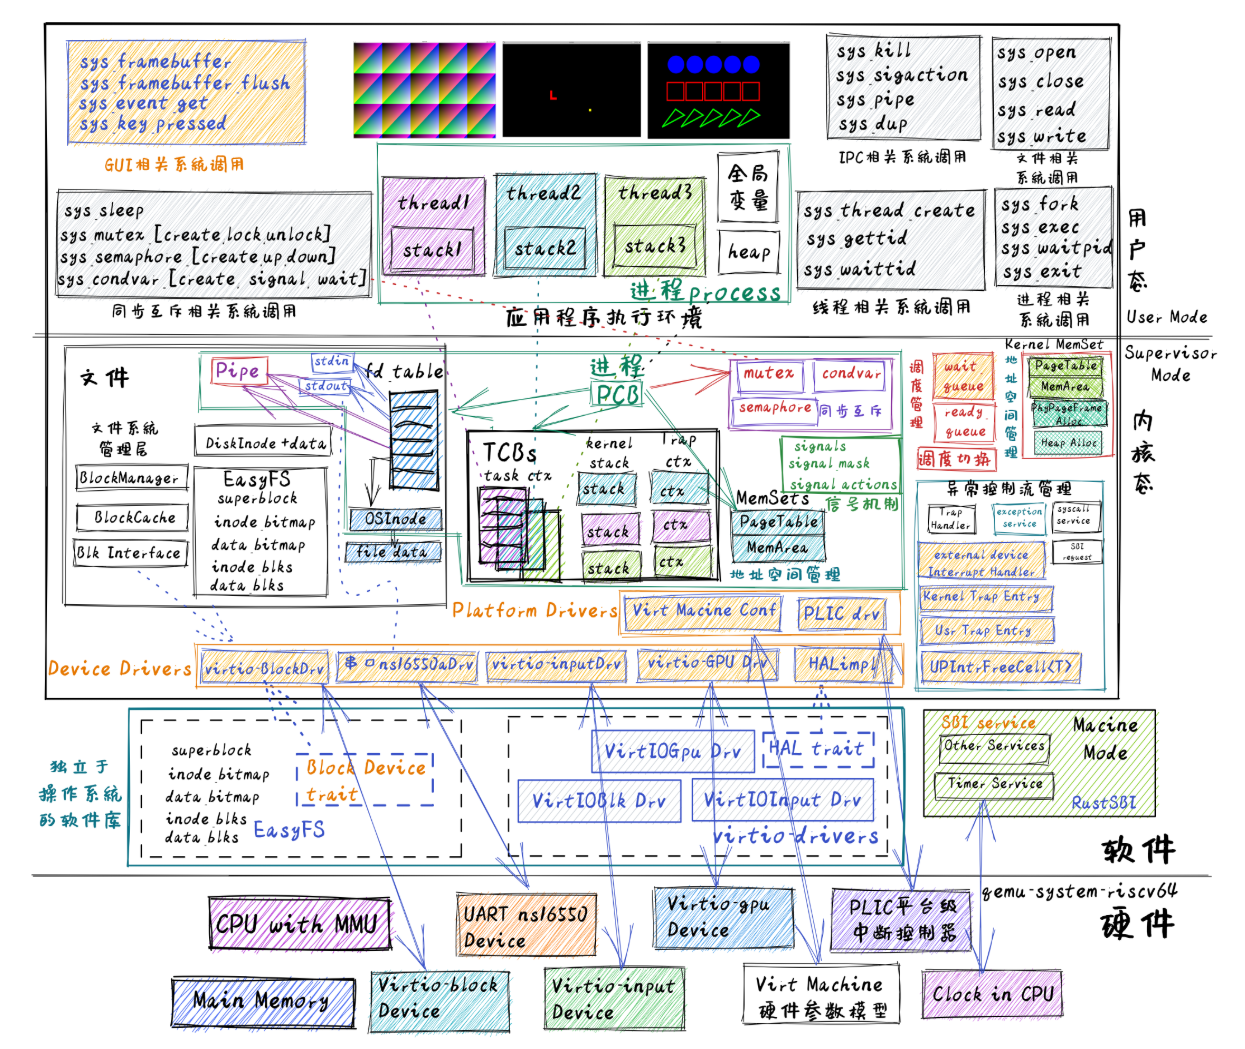
\includegraphics[width=1.0\textwidth]{../image/Architecture.png}
    \caption{系统架构图}
    \label{fig:architecture}
\end{figure}